%!TEX program = xelatex

\documentclass[11pt,titlepage]{report}
%!TEX root = main.tex

\usepackage[T1]{fontenc}
\usepackage{lmodern}
\usepackage[svgnames]{xcolor}
\usepackage{fontspec} % XeLaTeX required!
\usepackage{graphicx}
\usepackage{circuitikz}
\usepackage{tikz}
\usepackage{pifont}
\usepackage[some]{background}
\usepackage{xltxtra} 
\usepackage{setspace}
\usepackage[absolute]{textpos}
\usepackage[latin1]{inputenc}
\usepackage[english]{babel}
\usepackage{graphicx}
\usepackage{wrapfig}
\usepackage{fullpage}
\usepackage[margin=1in]{geometry}
\usepackage{float}
\usepackage{url}
\usepackage{multicol}
\usepackage{hyperref}
\usepackage{titlepic}
\usepackage{standalone}
\usepackage{siunitx}
\usepackage{booktabs}
\usepackage{amsmath}
\usepackage{unicode-math}
\usepackage{verbatim}
\usepackage{enumitem}
\usepackage{listings}
\usepackage{multirow}
\usepackage{pgfplots}
\pgfplotsset{compat=1.8}
\usepackage{caption} 
\usepackage[parfill]{parskip}
\usepackage{import}
\usepackage[backend=bibtexu,texencoding=utf8,bibencoding=utf8,style=ieee,sortlocale=en_GB,language=auto]{biblatex}
\usepackage[strict,autostyle]{csquotes}
\usepackage[final]{pdfpages}
\usepackage{subcaption}
\usepackage{ifplatform}
%\captionsetup[table]{skip=10pt}


% Fix for includepdf bug in Mac OS X
\newcommand{\insertpdfpath}[1]{
	\ifwindows
	\newcommand{\insertpdf}[2]{\includepdf[pages=##1]{##2}}
	\else
	\newcommand{\insertpdf}[2]{\includepdf[pages=##1]{#1/##2}}
	\fi
}

%set fonts
\setmainfont[Ligatures=TeX]{Myriad Pro}
\setmathfont{Asana Math}
\setmonofont{Lucida Console}

\usepackage{titlesec, color}
\renewcommand{\familydefault}{\sfdefault} %set font family
\renewcommand{\arraystretch}{1.2} %set table vertical spacing
\setlength\parindent{0pt} %no paragraph indent
\hypersetup{ %setup hyperlinks
    colorlinks,
    citecolor=black,
    filecolor=black,
    linkcolor=black,
    urlcolor=black
}

%redesign chapter headings
\definecolor{gray75}{gray}{0.75}
\newcommand{\chapternumber}{\thechapter}
\newcommand{\hsp}{\hspace{20pt}}
\titleformat{\chapter}[hang]{\Huge\bfseries}{\chapternumber\hsp\textcolor{gray75}{|}\hsp}{0pt}{\Huge\bfseries}

%Redefine appendix headers
\renewcommand{\appendixname}{Appendix}
\renewcommand{\appendixtocname}{Appendices}
\renewcommand{\appendixpagename}{Appendices}

%For code listings
\definecolor{black}{rgb}{0,0,0}
\definecolor{browntags}{rgb}{0.65,0.1,0.1}
\definecolor{bluestrings}{rgb}{0,0,1}
\definecolor{graycomments}{rgb}{0.4,0.4,0.4}
\definecolor{redkeywords}{rgb}{1,0,0}
\definecolor{bluekeywords}{rgb}{0.13,0.13,0.8}
\definecolor{greencomments}{rgb}{0,0.5,0}
\definecolor{redstrings}{rgb}{0.9,0,0}
\definecolor{purpleidentifiers}{rgb}{0.01,0,0.01}


\lstdefinestyle{csharp}{
language=[Sharp]C,
showspaces=false,
showtabs=false,
breaklines=true,
showstringspaces=false,
breakatwhitespace=true,
escapeinside={(*@}{@*)},
columns=fullflexible,
commentstyle=\color{greencomments},
keywordstyle=\color{bluekeywords}\bfseries,
stringstyle=\color{redstrings},
identifierstyle=\color{purpleidentifiers},
basicstyle=\ttfamily\small}

\lstdefinestyle{c}{
language=C,
showspaces=false,
showtabs=false,
breaklines=true,
showstringspaces=false,
breakatwhitespace=true,
escapeinside={(*@}{@*)},
columns=fullflexible,
commentstyle=\color{greencomments},
keywordstyle=\color{bluekeywords}\bfseries,
stringstyle=\color{redstrings},
identifierstyle=\color{purpleidentifiers},
}

\lstdefinestyle{matlab}{
language=Matlab,
showspaces=false,
showtabs=false,
breaklines=true,
showstringspaces=false,
breakatwhitespace=true,
escapeinside={(*@}{@*)},
columns=fullflexible,
commentstyle=\color{greencomments},
keywordstyle=\color{bluekeywords}\bfseries,
stringstyle=\color{redstrings},
identifierstyle=\color{purpleidentifiers}
}

\lstdefinestyle{vhdl}{
language=VHDL,
showspaces=false,
showtabs=false,
breaklines=true,
showstringspaces=false,
breakatwhitespace=true,
escapeinside={(*@}{@*)},
columns=fullflexible,
commentstyle=\color{greencomments},
keywordstyle=\color{bluekeywords}\bfseries,
stringstyle=\color{redstrings},
identifierstyle=\color{purpleidentifiers}
}

\lstdefinestyle{xaml}{
language=XML,
showspaces=false,
showtabs=false,
breaklines=true,
showstringspaces=false,
breakatwhitespace=true,
escapeinside={(*@}{@*)},
columns=fullflexible,
commentstyle=\color{greencomments},
keywordstyle=\color{redkeywords},
stringstyle=\color{bluestrings},
tagstyle=\color{browntags},
morestring=[b]",
  morecomment=[s]{<?}{?>},
  morekeywords={xmlns,version,typex:AsyncRecords,x:Arguments,x:Boolean,x:Byte,x:Char,x:Class,x:ClassAttributes,x:ClassModifier,x:Code,x:ConnectionId,x:Decimal,x:Double,x:FactoryMethod,x:FieldModifier,x:Int16,x:Int32,x:Int64,x:Key,x:Members,x:Name,x:Object,x:Property,x:Shared,x:Single,x:String,x:Subclass,x:SynchronousMode,x:TimeSpan,x:TypeArguments,x:Uid,x:Uri,x:XData,Grid.Column,Grid.ColumnSpan,Click,ClipToBounds,Content,DropDownOpened,FontSize,Foreground,Header,Height,HorizontalAlignment,HorizontalContentAlignment,IsCancel,IsDefault,IsEnabled,IsSelected,Margin,MinHeight,MinWidth,Padding,SnapsToDevicePixels,Target,TextWrapping,Title,VerticalAlignment,VerticalContentAlignment,Width,WindowStartupLocation,Binding,Mode,OneWay,xmlns:x}
}

\lstdefinestyle{matlab}{
language=Matlab,
showspaces=false,
showtabs=false,
breaklines=true,
showstringspaces=false,
breakatwhitespace=true,
escapeinside={(*@}{@*)},
columns=fullflexible,
commentstyle=\color{greencomments},
keywordstyle=\color{bluekeywords}\bfseries,
stringstyle=\color{purpleidentifiers},
identifierstyle=\color{purpleidentifiers}
}

%defaults
\lstset{
basicstyle=\ttfamily\small,
extendedchars=false,
numbers=left,
numberstyle=\ttfamily\tiny,
stepnumber=1,
tabsize=4,
numbersep=5pt
}
\addbibresource{../../library/bibliography.bib}

\begin{document}

\chapter{Localization}
\label{ch:localization}
An important sub section of the complete system is the localization of KITT. Not only is it important to know whether a waypoint has been reached, the entire control strategy of the car relies on accurate location information. To achieve this, a Time-Difference of Arrival (TDOA) method was employed using audio transmitted by the beacon mounted to the car and received by five microphones placed in the room.

Before the actual localization can take place, several steps must be taken to obtain the TDOAs. First, the transmitted signal must be specified. This is not quite trivial and is explained in section \ref{sec:loc_transmit}. Then, the difference in arrival times between the various microphones must be calculated. This is done by finding peaks (section \ref{sec:loc_peak}) in the propagation channel (section \ref{sec:loc_est_h}). Before the channel can be accurately estimated, it needs to be trimmed to meet specific criteria. These criteria are outlined in section \ref{sec:loc_data_trim}. Finally, once the TDOAs are known, they can be used to calculate the position of the sound source. The algorithm behind this is detailed in section \ref{sec:loc_alg}. Some future considerations which are not currently implemented are discussed in the last paragraph, section \ref{sec:loc_future}.

A general overview of the localization system is shown in figure \ref{fig:localization-overview}. The figure shows the generation of the deconvolution matrix, fed by reference measurements, in the initialization phase of the entire system. Inherent to the design, this matrix needs to be generated only once. The iterative behaviour is called continuously and eventually leads to the localization and angle determination.
\begin{figure}[H]
	\centering
	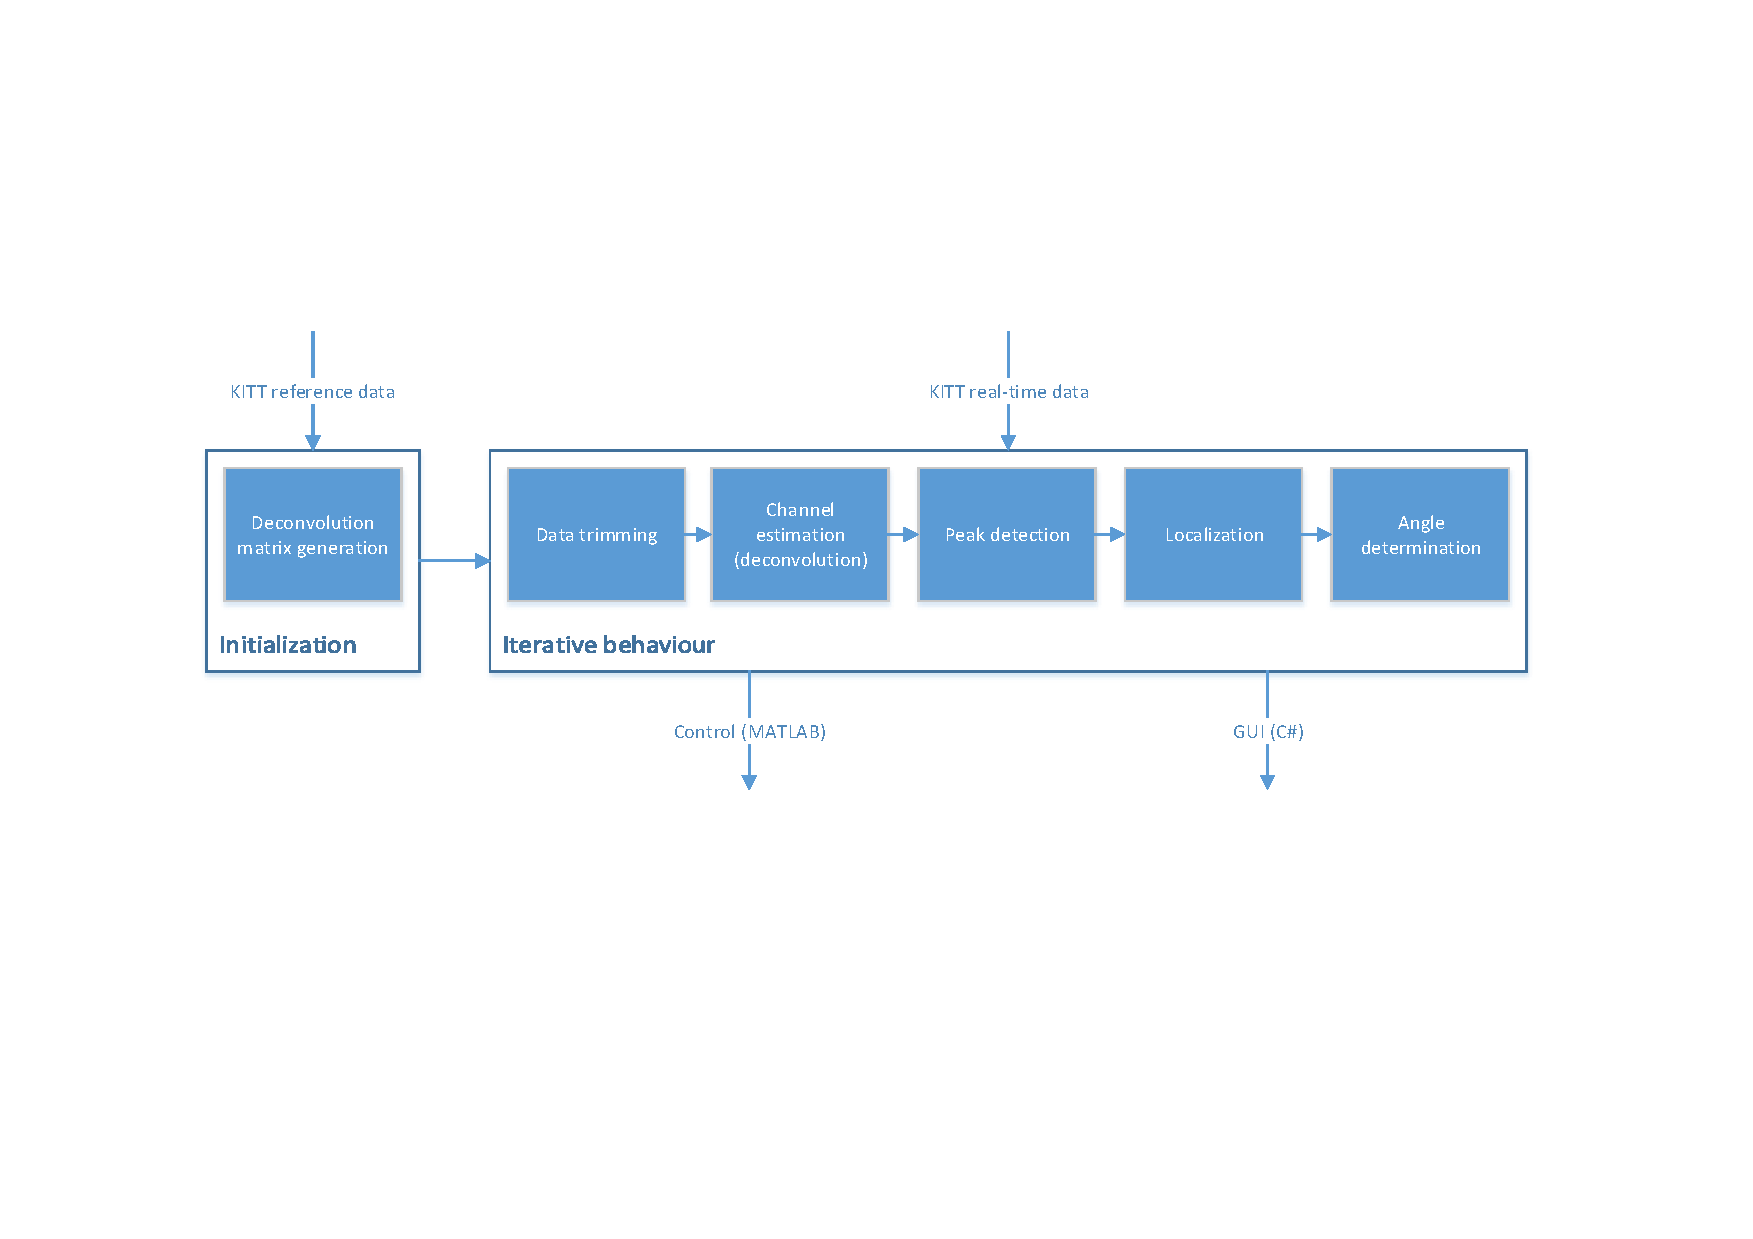
\includegraphics[width=\linewidth]{resource/localization-overview.pdf}
	\caption{The work flow of the designed localization system}
	\label{fig:localization-overview}
\end{figure}

\section{Transmitted signal}
\label{sec:loc_transmit}
As reported in \cite{epo4-del7} the main goal of the transmitted sequence is to be able to perfectly identify it under every circumstance; even in the presence of noise or signals emitted by other beacons. Only some parameters of the transmitted signal can be changed; for example it is already defined to be an OOK signal. The tweaking parameters are the carrier frequency, the code frequency, the repetition frequency and the code word (and thus its length). More details on the choice of the sequence is given in \cite{epo4-del7} but the conclusions are summarized in table \ref{tab:loc_signal}.

Using the given microcontroller programmer, the thus defined reference signal was programmed onto KITT.

% TODO fix this table!
\begin{table}[H]
\centering
\begin{tabular}{c | c | c}
\hline \hline
Parameter & Choice & Reasoning \\
\hline
Carrier frequency & \SI{15}{khz} & 
Chosen frequency is high enough to prevent most interference with human speech but low enough that the beacon can accurately represent it.\\
Code frequency & \SI{5}{khz} & High code frequency may lead to inaccurate measurements. This setting proved to work in practice.\\
Repeat frequency & \SI{8}{hz} & Higher repeat frequency guarantees more frequent localization but leaves less room between samples. In \cite{epo4-del7} it was shown that this setting is optimal.\\
Code word & \texttt{4eeb428c} & A randomly generated hexadecimal string.\\
\end{tabular}
\caption{Summary of chosen audio beacon parameters}
\label{tab:loc_signal}
\end{table}

\section{Recording and data trimming}
\label{sec:loc_data_trim}
The recording stage is the gateway between the physical sound and the digital signal processing. Each microphone is recorded using an audio interface connected via USB to the computer at a sample rate of \SI{48}{\kilo\hertz}. Since the localization should be done as often as possible to get accurate results, the recording process should take as little time as possible yet still guarantee the presence of a complete response. Therefore, the recording time was set to two times the repeat time, e.g. \SI{250}{\milli\second}. If the recording would start exactly at the first received peak, no data trimming would be necessary. But because the recording is not synchronized to the emitted sound we have no method of verifying this. Therefore the data must first be trimmed.

Data trimming is done for two reasons: \textbf{(1)}, the recorded data must not include sound sent by a previous pulse (ideally including reflections) and \textbf{(2)}, the signal we wish to deconvolve must be a causal response to the \SI{1}{\centi\meter} reference measurements. \textbf{(1)} was guaranteed by truncating the recording to a limited interval around the peak in the highest quality channel estimate. As a measure for channel quality $\frac{\text{max}(h[n])}{\text{std}(h[n])}$ was used since this gives a quick indication of the signal to noise ratio. Then, a similar peak detection algorithm as described in section \ref{sec:loc_peak} was used to find the peak value in the channel. The interval the signal was truncated to is given by the field dimensions: since the expectation is that KITT should not leave the field the maximum distance a sound pulse must travel is diagonally across the field. Since this distance is known (\SI{49}{\meter\squared}), the speed of sound is known (\SI{343}{\meter\per\second}) and the sample frequency of the audio interface is known (\SI{48}{\kilo\hertz}), the delay between peaks can be no more than \num{1400} samples. Further more, the highest quality signal is likely to be closer to a microphone so it makes sense not to \textit{center} the search interval around the peak sample, but to bias it more towards the samples following the peak. Therefore, calling the sample at which the highest quality peak is detected $t_0$ and allowing some headroom, the search interval was set to $[t_0 - 400, t_0 +1500]$.

\section{Channel estimation}
\label{sec:loc_est_h}
Channel estimation is done using matrix inversion as described in the manual \cite{epo4-manual}. The matched filter approach was also tested but proved to be less reliable because the obtained channel responses had no clear peak. Summarizing from \cite{epo4-manual} and \cite{epo4-del7}, a signal $y[n]=x[n]*h[n]$ is received at every microphone. The deconvolution method then approximates $h[n]$ as $\vec{\hat{h}}=(\mat{X}^T\mat{X})^{-1}\mat{X}^T\vec{y}$, where $\mat{X}$ is a matrix in Toeplitz form as outlined in \cite{epo4-manual}. Because the sent signal is known, the matrix $\mat{X}^\dagger=(\mat{X}^T\mat{X})^{-1}\mat{X}^T$ can be calculated beforehand. In practical implementations, this matrix must be computed for every microphone because the response of each matrix will vary slightly. Therefore, the matrix was computed for every microphone using recordings of the training sequence which were recorded at \SI{1}{cm} distance from that microphone.

The size of the resulting matrix $\mat{X}^\dagger$ is dependent on the amount of microphones used, the estimated length of the channel, $L$, and the length of the \SI{1}{cm} recordings, $N_x$. Because the number of microphones is fixed at \num{5}, the calculation of $\mat{X}^\dagger$ can only be sped up by reducing the size (and thus accuracy) of the deconvolution matrix and accuracy increased by increasing $L$ and $N_x$. This is a complicated trade-off that must be made and tailored to the hardware used. The used settings for KITT are $L=3500$ and $N_x=500$, which allow good deconvolution properties, but leaves $\mat{X}^\dagger$ to be calculated within a few minutes on modern computers.

A potential problem to the matrix inversion necessary for the calculation of $\mat{X}^\dagger$ is when the matrix $\mat{A}=\mat{X}^T\mat{X}$ is singular or ill-conditioned. When $\mat{A}$ is singular (the determinant of $\mat{A}$ is zero), $\mat{X}^\dagger$ cannot be calculated and when $\mat{A}$ is ill-conditioned\footnote{A matrix is said to be ill-conditioned if the ratio of the largest singular value to the smallest singular value (the condition number) $c=\frac{\sigma_1}{\sigma_n}$ is `large'. Though `large' is not well-defined itself, it can be shown \cite{epo4-manual} that an error $\epsilon$ in the input to a linear system is potentially magnified by the condition number in the solution.} the resulting matrix is dominated by small singular values. In order to overcome this potential problem, a singular value filter was built into the matrix inversion algorithm. The filter works as follows:
Let $\mat{A}=\mat{U}\mat{\Sigma}\mat{V}^T$ be the singular value decomposition of $\mat{A}=\mat{X}^T\mat{X}$ where $\mat{A}$ is of size $m\times n$. Then $\mat{\Sigma}$ is a diagonal matrix of size $m \times n$ containing the singular values $\sigma_1, \sigma_2, ..., \sigma_n$ of $\mat{A}$ on the diagonal in descending order. For any $\sigma_i<t$, where $t$ is some threshold, the left inverse of $\mat{A}$ is approximated by $\mat{\hat{A}}^\dagger=\mat{\hat{V}}\mat{\hat{\Sigma}}^{-1}\mat{\hat{U}}^T$ where $\mat{\hat{V}}$, $\mat{\hat{\Sigma}}$ and $\mat{\hat{U}}$ are their respective matrices as defined before with the $i^\text{th}$ columns removed. 

The choice of threshold $t$ is non-trivial and was determined using trial and error on measurement data. We discovered that the `optimal' threshold was slightly different for each microphone and even each measurement. An important insight is that when the threshold is set too high, e.g. too large singular values are filtered, some calculated channel responses are no longer identifiable as such. Specifically, the result would be a modulated sine wave. In order to prevent this from happening during the demonstration, the thresholds for each microphone channel were chosen somewhat conservative, see table \ref{tab:loc_svd_value}.

% TODO: check values in table
% TODO: include reference to channel estimation matlab

\begin{table}[H]
\centering
\begin{tabular}{ c | c}
\hline \hline
Microphone channel & Singular value threshold $t$ \\
\hline
1 & \num{0.1} \\ 
2 & \num{0.2} \\
3 & \num{0.5} \\
4 & \num{0.2} \\
5 & \num{0.015} \\
\end{tabular}
\caption{Singular value threshold for each microphone channel}
\label{tab:loc_svd_value}
\end{table}

\section{Peak detection}
\label{sec:loc_peak}
The previous report \cite{epo4-del7} described two methods of localizing the peaks in the estimated channel, the first based on \texttt{MATLAB}'s \texttt{findpeaks} function and the second based on smart utilization of the standard deviation of the channel. However, after revising the code it seemed both these approaches were too time consuming. It was decided instead to implement a simpler detection algorithm which simply scans the estimated channel sample by sample and compares the amplitude to some threshold which is proportional to the maximum of all samples. After some simple testing on synthetic data this turned out to be up to a factor \num{40} faster than the \texttt{findpeaks} implementation. Since the standard deviation approach was already at least a factor \num{10} slower than the \texttt{findpeaks} algorithm, it was decided to use the threshold approach. 
% TODO insert reference to find_start.m
A plot of an arbitrary recovered impulse response is shown in figure \ref{fig:localization-typical-impulse}. In green the work of the peak detection algorithm is shown. 

\begin{figure}[H]
	\centering
	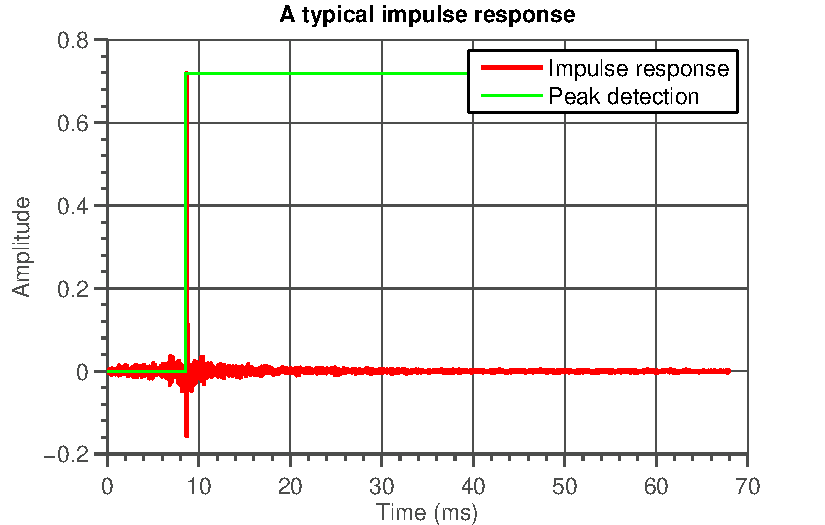
\includegraphics[width=0.5\linewidth]{resource/typical-impulse.pdf}
	\caption{A typical impulse response along with the detected peak}
	\label{fig:localization-typical-impulse}
\end{figure}

\section{Localization algorithm}
\label{sec:loc_alg}
Once the peaks have been detected in all five microphone channels, a range difference matrix can be constructed consisting of entries $r(i,j)$ corresponding to the range difference between microphones $i$~and~$j$. Obviously, the diagonal is zero. 
% TODO: add reference to getrangematrix.m
Using the range difference matrix $\mat{R}$ we can construct a matrix $\mat{A}$, a vector $\vec{x}$ and a vector $\vec{b}$ as in \cite{epo4-manual}, $\mat{A}\vec{x}=\vec{b}$ rows of $\mat{A}$ are constructed for each microphone pair $(i,j)$ as
\begin{equation}
\begin{bmatrix}
2(\vec{x}_j-\vec{x}_i)^T & -2r_{i,j}
\end{bmatrix}
\end{equation}

The entries of vector $\vec{b}$ are also constructed for each microphone pair as
\begin{equation}
\begin{bmatrix}
r_{i,j}^2-||\vec{x}_i||^2+||\vec{x}_j||^2
\end{bmatrix}
\end{equation}

The vector $\vec{x}$ that solves these equations may not exist because the system is overdetermined: there are \num{5} microphones (so $\mat{A}$ has \num{10} rows) and we limit ourself to two coordinates yielding \num{6} columns in $\mat{A}$. Therefore, the solution $\vec{x}$ is calculated (much in the same way as in section \ref{sec:loc_est_h}) as the solution of the matrix equation $\mat{A}\vec{x}=\vec{b}$ in an ordinary least squares way: $\vec{x}=(\mat{A}^T\mat{A})^{-1}\mat{A}^T\vec{b}$. This method yields an exact solution if it exists and otherwise produces the $\vec{x}$ with the least squares error. The first two entries of $\vec{x}$ are the resulting position of KITT. 
% TODO: include reference to localize.m

The angle at which KITT is driving through the field, $\theta$, can be calculated from the current and previous location. Let $\vec{x}_n=\begin{bmatrix}x_n\\y_n\end{bmatrix}$ be the latest determined position and $\vec{x}_{n-1}=\begin{bmatrix}x_{n-1}\\y_{n-1}\end{bmatrix}$ the previous location, then $\theta$ is given by
\begin{equation}
\theta = \tan^{-1}\left(\frac{y_n-y_{n-1}}{x_n-x_{n-1}}\right)
\end{equation}




\section{Future work}
\label{sec:loc_future}
The subsections below explain some ideas we had floating in our head which did not make the final project due to time constraints, uncertainties about the implementation or superfluousness. 
\subsection{QR decomposition}
To improve numerical stability and accuracy, the least squares solutions presented in section \ref{sec:loc_est_h} and \ref{sec:loc_alg} can be performed using the QR decomposition. Generally, letting $\mat{A}\vec{x}=\vec{b}$ be the overdetermined system, trying to minimize $||\mat{A}\vec{\hat{x}}=\vec{b}||$ can be done using the QR factorization: $\mat{A}=\mat{Q}\mat{R}$. The least squares solution is then $\hat{\vec{x}}=\mat{R}_1^{-1}\mat{Q}_1^T\vec{b}$. In this, $\mat{Q_1}$ and $\mat{R_1}$ are the \textit{economy size} versions of $\mat{Q}$ and $\mat{R}$ given by the \texttt{MATLAB} command \texttt{[Q, R] = qr(A,0)}. Although it might seem ineffici\"ent to factorize $\mat{A}$ and then invert $\mat{R}_1$, it can be shown \cite{num-methods} that $\mat{R}_1^{-1}$ does not need to be explicitly calculated because back-substitution may be used. Thus, making use of QR factorization in both the channel estimation and localization algorithm could speed up these processes.
\end{document}